\section{Background}
\label{sec:background}

\subsection{LLM Inference}
\label{sec:inference-background}

Autoregressive LLM inference has two execution phases (Figure~\ref{fig:inference-pipeline})~\cite{kwon2023vllm,zhong2024distserve,patel2024splitwise,strati2024dejavu}. During \emph{prefill}, the model processes all prompt tokens in parallel and materializes their key--value (KV) states. Prefill typically exposes substantial matrix-multiplication parallelism and is therefore compute intensive. During \emph{decode}, the model generates one token per iteration while reading the weights and an expanding KV cache. Decode consequently has lower arithmetic intensity and is often constrained by memory capacity and bandwidth. Time to first token (TTFT) captures prompt-processing and queueing delay, whereas time per output token (TPOT) and inter-token latency (ITL) capture decode responsiveness. Input/output lengths, batching, and offered load change the balance between these phases and thus their performance and energy behavior.

\begin{figure}[t]
  \centering
  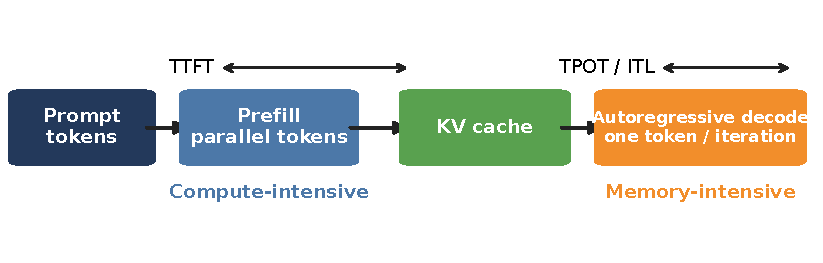
\includegraphics[width=\columnwidth]{figure/llm_inference_pipeline.pdf}
  \caption{The prefill and autoregressive decode phases of LLM inference.}
  \label{fig:inference-pipeline}
\end{figure}

\subsection{Parallel Deployment of LLMs}
\label{sec:parallelism-background}

Large models and high request rates require multiple GPUs. Figure~\ref{fig:parallelism} illustrates the three parallel dimensions considered in this work~\cite{shoeybi2019megatron,rajbhandari2022deepspeedmoe,zhang2026distributedenergy,wu2024loongserve,su2025seesaw}. Data parallelism (DP) replicates the model and partitions requests among replicas, increasing aggregate throughput at the cost of replicated weights. Tensor parallelism (TP) shards tensors or operators across GPUs and uses collectives to combine partial results; it reduces per-GPU memory demand but adds communication to each layer. Expert parallelism (EP) distributes MoE experts across GPUs and uses token dispatch and combine communication around routed FFN computation. Real deployments often combine DP, TP, and EP. Their compute utilization, memory footprint, and communication volume differ, so the fastest or lowest-power plan is not necessarily the most energy-efficient one.

\begin{figure}[t]
  \centering
  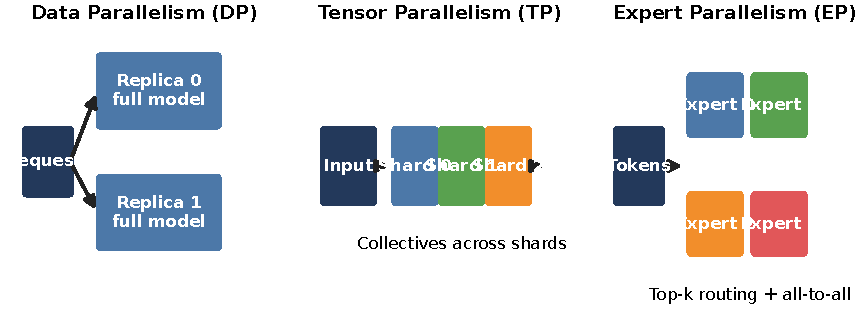
\includegraphics[width=\columnwidth]{figure/parallelism_dp_tp_ep.pdf}
  \caption{DP replicates models, TP shards operators, and EP distributes routed experts.}
  \label{fig:parallelism}
\end{figure}

\subsection{Disaggregated Serving Architectures}
\label{sec:disaggregation-background}

A conventional Native deployment executes prefill, decode, attention, and FFN computation in the same worker group. Prior systems introduced PD for phase-specialized serving and AF for disaggregated expert execution~\cite{zhong2024distserve,zhu2025megascale,patel2024splitwise,strati2024dejavu,lin2024infinitellm}. Disaggregation separates components with different resource characteristics so that they can be provisioned and scaled independently (Figure~\ref{fig:architectures}). Prefill--decode disaggregation (PD) assigns the two inference phases to separate pools and transfers request state and KV data from prefill workers to decode workers. Attention--FFN disaggregation (AF) separates the attention/KV path from dense or expert FFN computation and exchanges activations at transformer-layer boundaries. PD can match compute-oriented prefill with memory-oriented decode resources, while AF can specialize resources for attention and FFN. Both, however, introduce communication, synchronization, and pipeline overhead; whether separation saves energy depends on workload shape, parallel placement, and the underlying interconnect.

\begin{figure}[t]
  \centering
  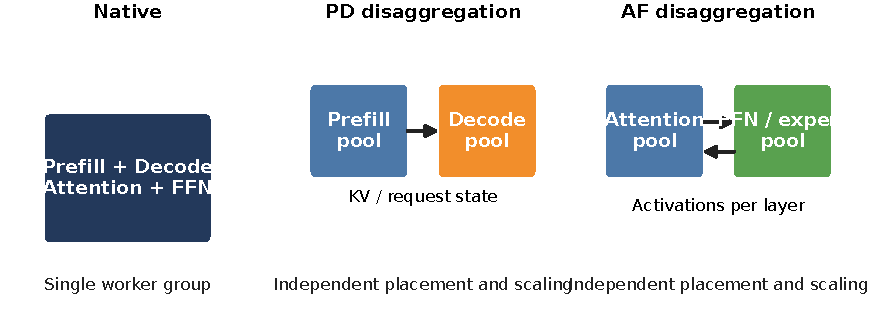
\includegraphics[width=\columnwidth]{figure/serving_architectures.pdf}
  \caption{Native, prefill--decode (PD), and attention--FFN (AF) serving architectures.}
  \label{fig:architectures}
\end{figure}

\subsection{Energy Management for LLM Serving}
\label{sec:energy-background}

Energy is the integral of power over execution time. A lower power draw therefore does not guarantee lower energy if it also extends request processing. Modern GPUs expose several control mechanisms, including core and memory dynamic voltage and frequency scaling (DVFS), power caps, and device consolidation~\cite{stojkovic2025dynamollm,kakolyris2025throttll,basit2026biscale,wang2025using,chung2025mlenergy}. Serving systems additionally control batching, placement, parallelism, and replica count. As shown in Figure~\ref{fig:energy-management}, an energy manager observes workload and system state, selects hardware and serving controls, and receives feedback through latency, throughput, power, and energy measurements. Useful policies must preserve TTFT/TPOT objectives while minimizing joules per request or maximizing tokens per joule. The best setting is architecture dependent because Native, PD, and AF expose different compute slack, memory traffic, and communication stalls.

\begin{figure}[t]
  \centering
  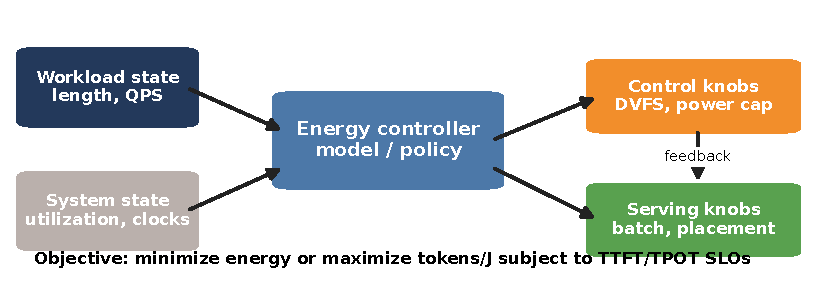
\includegraphics[width=\columnwidth]{figure/energy_management_loop.pdf}
  \caption{Closed-loop energy management for SLO-constrained LLM serving.}
  \label{fig:energy-management}
\end{figure}

\subsection{Datacenter and Consumer GPUs}
\label{sec:gpu-background}

GPUs used for LLM inference broadly fall into datacenter and consumer classes. Datacenter GPUs are designed for sustained multi-user operation and typically emphasize large error-correcting memory, predictable thermal behavior, remote manageability, virtualization, and high-speed scale-up or scale-out communication. Depending on the product family, they may provide NVLink/NVSwitch, GPUDirect RDMA, Multi-Instance GPU support, and stable power or clock controls. These features make datacenter GPUs suitable for multi-GPU serving and for deployments in which communication, availability, and isolation are first-order concerns~\cite{nvidiaA800datasheet,nvidiaL40Sspec,nvidiaL20spec}.

Consumer GPUs target interactive graphics and workstation workloads. They can offer high arithmetic throughput and favorable acquisition cost, but generally provide less memory, lack datacenter features such as NVLink and MIG, and have different cooling, reliability, and management assumptions. For example, the RTX~5090 exposes high Tensor throughput and fast GDDR7 memory but is a PCIe device without NVLink~\cite{nvidiaRTXBlackwell}. Consequently, peak FLOPS alone do not determine suitability for LLM serving: model capacity, memory behavior, communication requirements, power limits, and operational constraints all affect performance and energy efficiency. This distinction motivates evaluating both datacenter and consumer GPU classes rather than extrapolating conclusions from a single platform.
